\documentclass[11pt, aspectratio=169]{beamer}
\usetheme{Boadilla}
\usepackage{ragged2e}
\usepackage[utf8]{inputenc}
\usepackage{amsmath}
\usepackage{amsfonts}
\usepackage{amssymb}
\usepackage{textpos}
\usepackage{tabularx}
\usepackage{picture}
\usepackage{rotating}
\usepackage{textpos}
\usepackage{listings}
\usepackage{tikz}
\usetikzlibrary{calc}
\usetikzlibrary{positioning}
\usetikzlibrary{decorations.text}
\usetikzlibrary{decorations.pathmorphing}
\usepackage{mathtools}
\usepackage{rotating}
\usepackage{pgfplots}
\usepackage{multirow}
\usepackage{graphicx}
\usepackage{hyperref}
%\usepackage{multimedia}
\usepackage{movie15}
\usepackage{decorule}
\definecolor{navyblue}{rgb}{0.0, 0.2, 0.6}
\definecolor{olive}{rgb}{0.3, 0.66, 0.4}

\newsavebox{\myrule}
\sbox{\myrule}{\tikz {\path [fill, draw, color=navyblue] (0,0) [out=0, in=180] to +(.225\textwidth,1pt) [out=0, in=180] to +(.225\textwidth,-1pt) [out=180, in=0] to +(-.225\textwidth,-1pt) [out=180, in=0] to cycle;}}
\graphicspath{{figs/}}
\def\checkmark{\tikz\fill[scale=0.4](0,.35) -- (.25,0) -- (1,.7) -- (.25,.15) -- cycle;} 
\usetikzlibrary{arrows,shapes.geometric,positioning}
\usepackage{pifont}% http://ctan.org/pkg/pifont
\newcommand{\xmark}{\ding{55}}%
\definecolor{darkolivegreen}{rgb}{0.33, 0.62, 0.18}
% Define block styles
\usetikzlibrary{arrows.meta}
\usepackage{varwidth}
\tikzstyle{block} = [rectangle, draw, fill=blue!20, 
    text width=9.5em, text centered, rounded corners, minimum height=4em]
\tikzstyle{line} = [draw, -latex]
\renewcommand{\thempfootnote}{\arabic{mpfootnote}}
%\AtBeginSection{%
%\begin{frame}[noframenumbering]
 %   \tableofcontents%[currentsection, subsectionstyle=show/hide/show]
%\end{frame}
%} 
\addtobeamertemplate{footnote}{\hsize\textwidth}{}
%%%%%%%%%%%%%%%%%%
\definecolor{navyblue}{rgb}{0.0, 0.2, 0.6}
\author[Weiyao Ke]{}
\title[JETSCAPE Summer School 2020]{}
\begin{document}
\date[July, 2020]{}
\begin{frame}
\vspace{2.5em}
\begin{center}
{\Large  \color{navyblue} \bf JETSCAPE Framework for Medium Evolution} \\ 
%\decorule
\usebox{\myrule}\\
\vspace{.5em}
{\Large \color{navyblue} Initial collision geometry from the T\raisebox{-.3em}{R}ENTo}\\
\vspace{1em}
Weiyao Ke (UCB/LBNL)
\end{center}

\begin{center}
\begin{minipage}{.2\textwidth}

\includegraphics[width=\textwidth]{jetscape-logo.jpeg}
\end{minipage}\\
\begin{minipage}{.6\textwidth}
\begin{center}
{\color{gray} \footnotesize The JETSCAPE collaboration is supported by National Science Foundation under Cooperative Agreement ACI-1550300.}
\end{center}
\end{minipage}
\end{center}

\end{frame}

\begin{frame}
\tableofcontents
\end{frame}

\section{Introduction}
\begin{frame}{The JETSCAPE framework for medium evolution in heavy-ion collisions}
JETSCAPE\footnote{\href{http://jetscape.org/}{http://jetscape.org/}}: modular event generator for {\bf jet} and {\bf medium evolution} in relativistic heavy-ion collision. Develop statistical package to calibrate model parameters.
\begin{center}
\includegraphics[width=.85\textwidth]{flowchart2.pdf}
\end{center}
\end{frame}


\begin{frame}{Initializing the dynamical evolution of QGP}

\vspace{-1.7cm}
\begin{tikzpicture}
\node(A) at (0,0) {
\includegraphics[height=.5\textheight]{0.png}};
\node(B) at (0,-1.7) {
\includegraphics[height=.5\textheight]{1.png}};
\node(C) at (0,-3.5) {
\includegraphics[height=.5\textheight]{2.png}};
\node(D) at (0,-5.5) {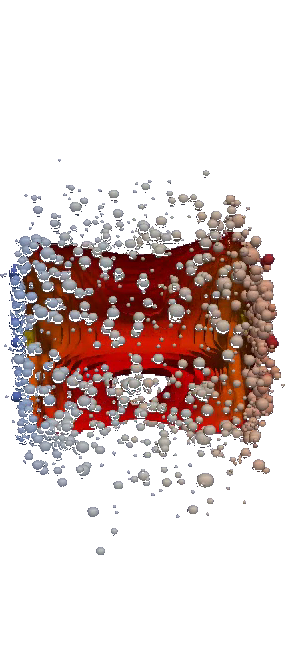
\includegraphics[height=.5\textheight]{4.png}};

\node(A1) at (8,0) {
\begin{varwidth}{.8\linewidth}

\vspace{1cm}
\begin{itemize}
\item Two approaching, Lorentz-contracted, nuclei $A$ and $B$.
\begin{itemize}
\item Nucleonic d.o.f. are slow and ``freeze'' on the collision time scale.
\item An event-by-event fluctuating nuclear geometry.
\end{itemize}
\end{itemize}
 \end{varwidth}
};
\node(B1) at (8,-1.7) {
    \begin{varwidth}{.8\linewidth}
    
    \vspace{1cm}
    \begin{itemize}
       \item Initial collisions: complicated many-body dynamics,  needs modeling.
      \begin{itemize}
      \item Simplication: only model energy depositon production at $\tau\rightarrow 0^+$.
\item What is the {\bf theoretical uncertainty} of a parametric $\frac{d E_T}{dx_\perp^2 d\eta_s}$?
\end{itemize}
\end{itemize}
    \end{varwidth}
};
\node(C1) at (8,-3.5) {
    \begin{varwidth}{.8\linewidth}
    
        \vspace{1cm}
    \begin{itemize}
      \item Early-time dynamics.
      \begin{itemize}
      \item A 3+1D freestreaming model.
      \item Evolve initial energy density.
      \end{itemize}
   \end{itemize}
      \end{varwidth}
};
\node(D1) at (8,-5.5) {
    \begin{varwidth}{.8\linewidth}
    
      \vspace{1cm}
      \begin{itemize}
      \item Relativistic viscous hydrodynamics.
      \begin{itemize}
      \item Matching energy-momentum tensor from early-time dynamics
      \end{itemize}
      \end{itemize}
      \end{varwidth}
};
\draw[->] (A)--(A1.west);
\draw[->] (B)--(B1.west);
\draw[->] (C)--(C1.west);
\draw[->] (D)--(D1.west);
\end{tikzpicture}
\end{frame}


\section{Review of medium evolution model}
\begin{frame}{The TRENTo initial condition model\footnote{http://qcd.phy.duke.edu/trento/index.html}: nuclear configuration}
\begin{columns}
\begin{column}[c]{.35\textwidth}
\begin{center}
\includegraphics[width=.45\textwidth]{lead_208.pdf}
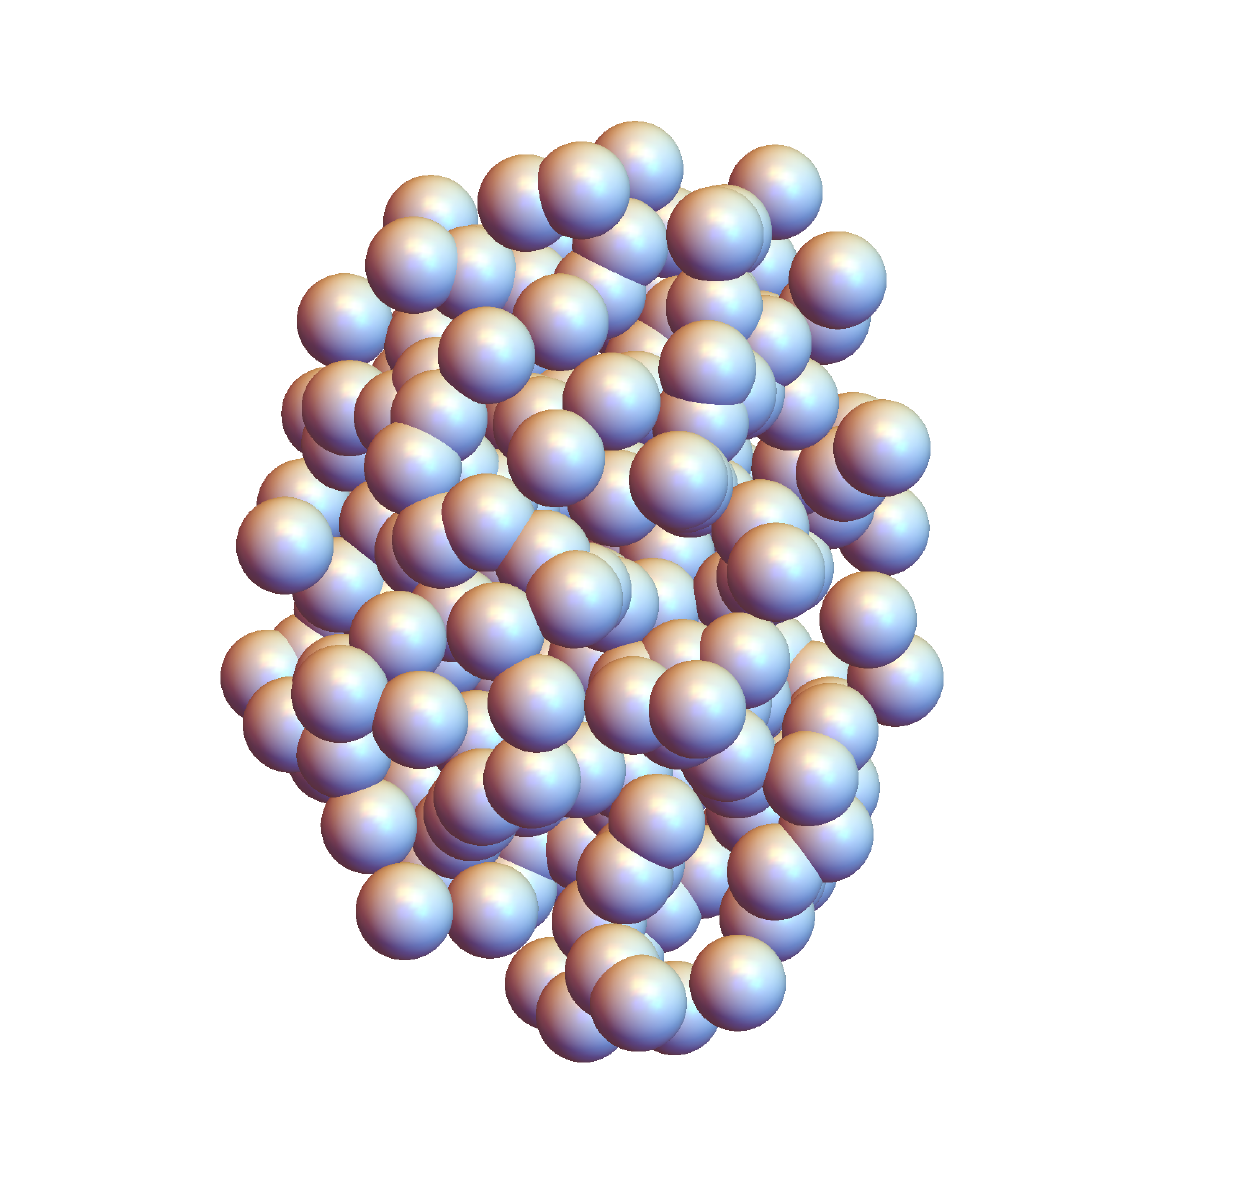
\includegraphics[width=.5\textwidth]{U_238.png}\\
{${}^{208}$Pb\quad\quad\quad\quad ${}^{238}$U}\\
\includegraphics[width=.45\textwidth]{lead_3.pdf}
\includegraphics[width=.45\textwidth]{lead_1.pdf}\\
{${}^{3}$He\quad\quad\quad\quad\quad p}
\end{center}
\end{column}
\begin{column}[c]{.65\textwidth}
\begin{itemize}
\item Sample nucleon positions according to the (deformed) Woods-Saxon distribution of heavy nuclei\footnote{Woods Saxon parameters from .For light nuclei like ${}^3$He, one can use configurations generated by nuclear structure calculation}, 
\begin{eqnarray}
\nonumber
\frac{dN}{dr d\Omega} &\propto& \frac{1}{1+e^{\frac{r-r_0(\theta, \phi))}{a}}},
\\\nonumber
r_0(\theta, \phi) &=& R(1+\beta_2 Y_{20} + \beta_4 Y_{40})
\end{eqnarray}
\begin{itemize}
\item $\beta_2, \beta_4$ nuclear quadruple and hexadecapole moments.
\item $R$: radius parameter.
\item $a$: diffusiveness parameter.
\end{itemize}
\item Sample with minimum nucleon-nucleon distance $d_{\min}$ to mimic short-range repulsion.
\end{itemize}
\end{column}
\end{columns}
\end{frame}


\begin{frame}{Nucleon profile and pairwise nucleon inelastic collisions}
\begin{columns}
\begin{column}[c]{.35\textwidth}
\begin{tikzpicture}
\node(A) at (0,0) {\includegraphics[width=\textwidth]{pp_overlap.pdf}};
\draw[<->] (-.5,-.5)--(.5,-.5);
\node(B) at(-.7,.5){$\rho_p(r)$};
\node(C) at(+.7,.5){$\rho_p(r)$};
\node(D)at(0,-.8){$b$};
\end{tikzpicture}
\begin{center}
\vspace{-1em}
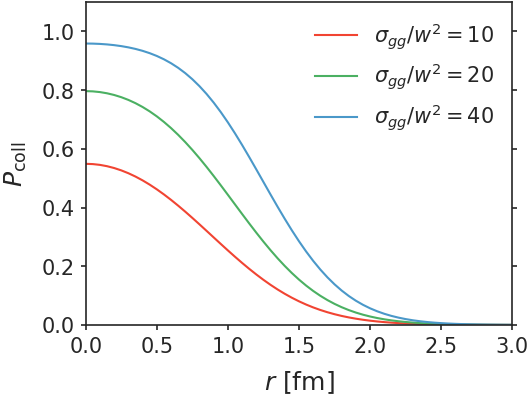
\includegraphics[width=\textwidth]{Pcoll.png}
\end{center}
\end{column}
\begin{column}[c]{.65\textwidth}
\begin{itemize}
\item 3D Gaussian model of proton density
\vspace{-.5em}
\begin{eqnarray}
\nonumber
\rho_p(r, z) = \frac{e^{-\frac{r^2+z^2}{2w^2}}}{(2\pi w)^{3/2}} 
 \xrightarrow{\textrm{Projection}} \rho_p(r) = \frac{e^{-\frac{r^2}{2w^2}}}{2\pi w^2} 
\end{eqnarray}
\item Probability of two nucleons to collide depends on the density overlap $T_{pp}(b)$, $b$ is the impact parameter.
\vspace{-.5em}
\begin{eqnarray}
\nonumber
T_{pp}(b) &=& \int \rho_p(r-b/2) \rho_p(r+b/2) dr^2 
\\
\nonumber
P_{\textrm{coll}}(b) &=& 1-\exp\left\{  -\sigma_{gg} T_{pp}(b) \right\}
\end{eqnarray}
\item $\sigma_{gg}$: an effective opacity parameter tuned to reproduce the $pp$ inelastic cross-section at given beam energy ($\sqrt{s}$)
\begin{eqnarray}
\nonumber
\sigma_{\textrm{inel}}(\sqrt{s}) = \int P_{\textrm{coll}}(b; \sigma_{gg}(\sqrt{s})) db^2 \rightarrow \frac{\sigma_{gg}}{w^2} = f\left( \frac{\sigma_{NN}}{w^2}\right)
\end{eqnarray}
\end{itemize}
\end{column}
\end{columns}
\end{frame}

\begin{frame}{Participants and binary collisions}
\begin{columns}
\begin{column}{.3\textwidth}
\begin{overprint}
\onslide<1>
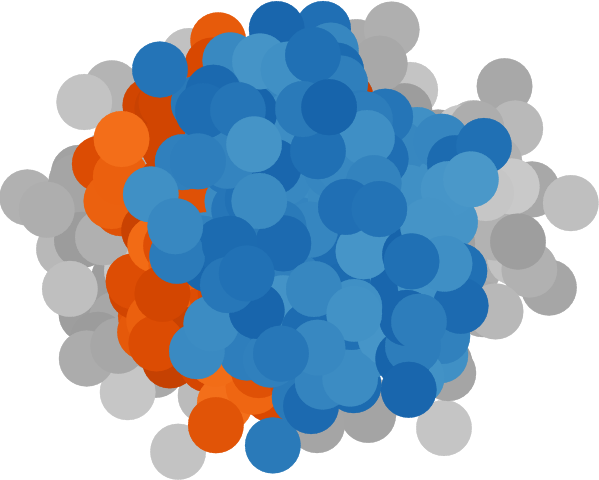
\includegraphics[width=\textwidth]{Participants.png}
\onslide<2>
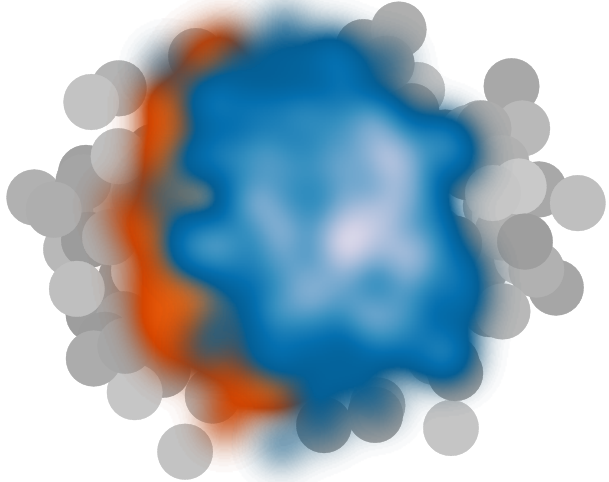
\includegraphics[width=\textwidth]{Npart-density.png}
\end{overprint}
\end{column}
\begin{column}{.7\textwidth}
\begin{itemize}
\item Check each pair of nucleons $(i,j)$ from the two collision nuclei $A$ and $B$ separated by impact-parameter $b$,
\begin{eqnarray}
\nonumber
\textrm{Collide with probability }P_{\textrm{coll}}(\mathbf{r}_j+\mathbf{b}-\mathbf{r}_i)
\end{eqnarray}
\item Participants: nucleons suffer at lease one inelastic collisions. 
\item<2-> Smoothed participant density:
\begin{eqnarray}
\nonumber
T_{A \textrm{ or }B}(\mathbf{r}) = \sum_{i\in \textrm{Part. $A$ or $B$}} \gamma_i \rho_p(\mathbf{r}-\mathbf{r}_i)
\end{eqnarray}
\item<2-> $\gamma_i$ draw from $\Gamma$ distribution $\sim \gamma^{k-1} e^{-k\gamma}$. Important to simulate huge multiplicity fluctuation in $pp$ collisions.
\end{itemize}
\end{column}
\end{columns}
\end{frame}

\begin{frame}{Energy density production at mid-rapidity}
\begin{columns}
\begin{column}{.35\textwidth}
\begin{overprint}
\onslide<1>
\begin{center}
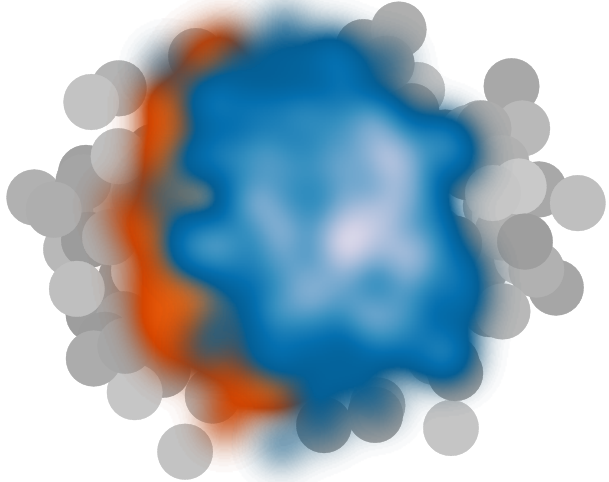
\includegraphics[width=.7\textwidth]{Npart-density.png}\\
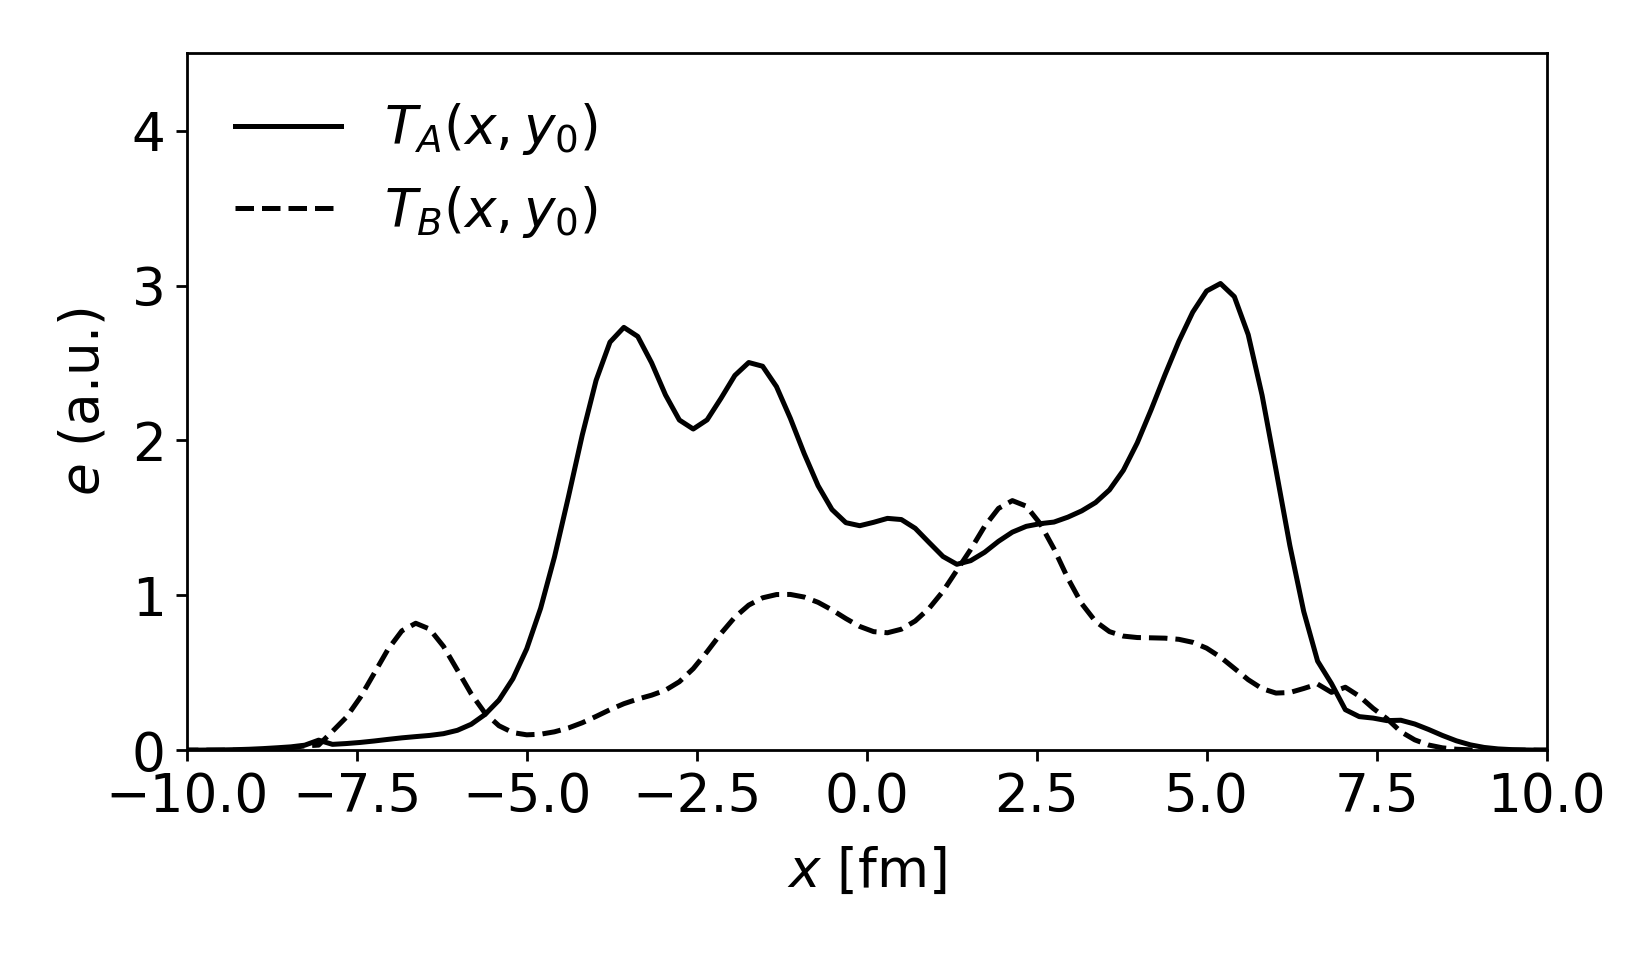
\includegraphics[width=\textwidth]{trento_p_tatb.png}
\end{center}
\onslide<2>
\begin{center}
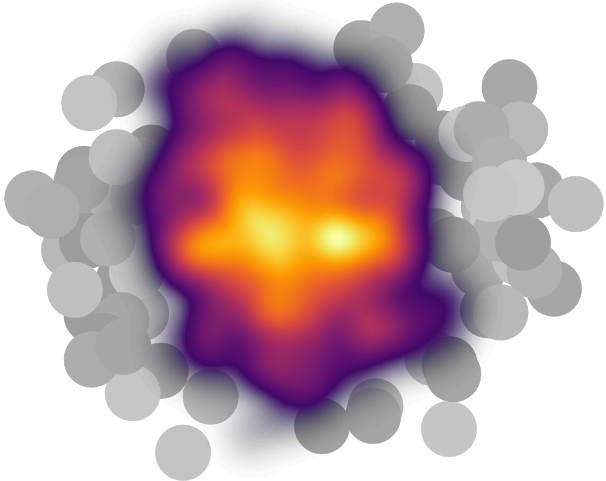
\includegraphics[width=.7\textwidth]{s-density.png}\\
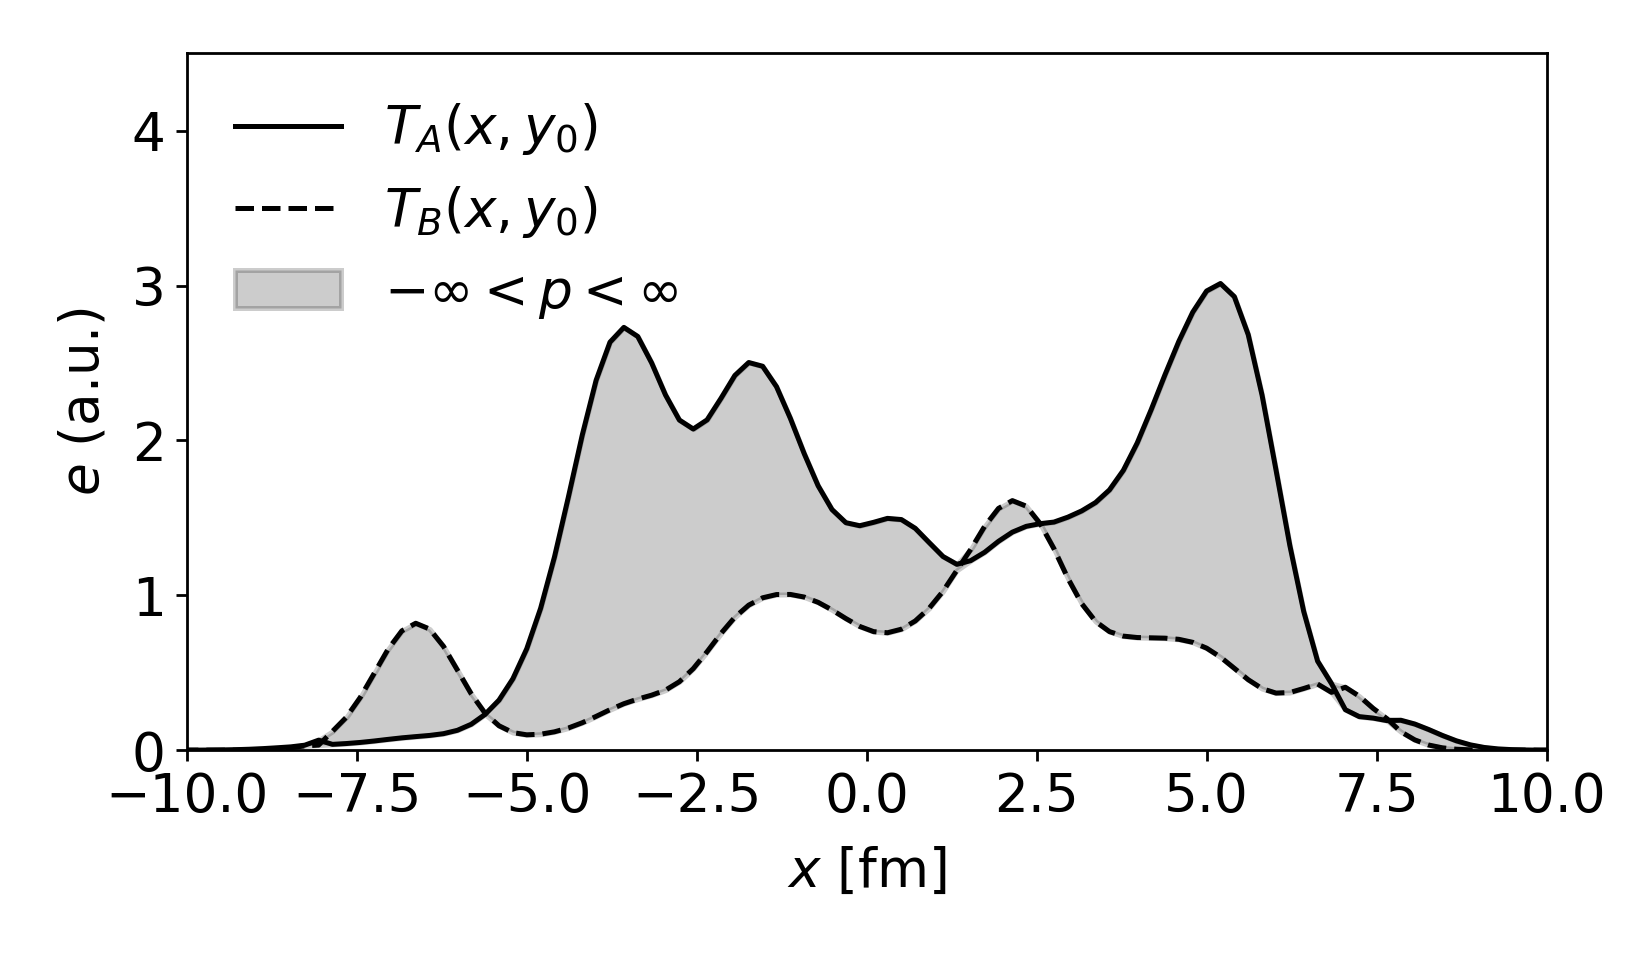
\includegraphics[width=\textwidth]{trento_p_allp.png}
\end{center}
\onslide<3>
\begin{center}
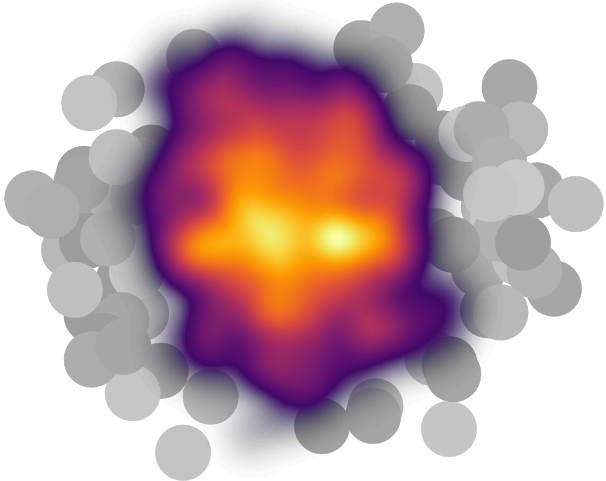
\includegraphics[width=.7\textwidth]{s-density.png}\\
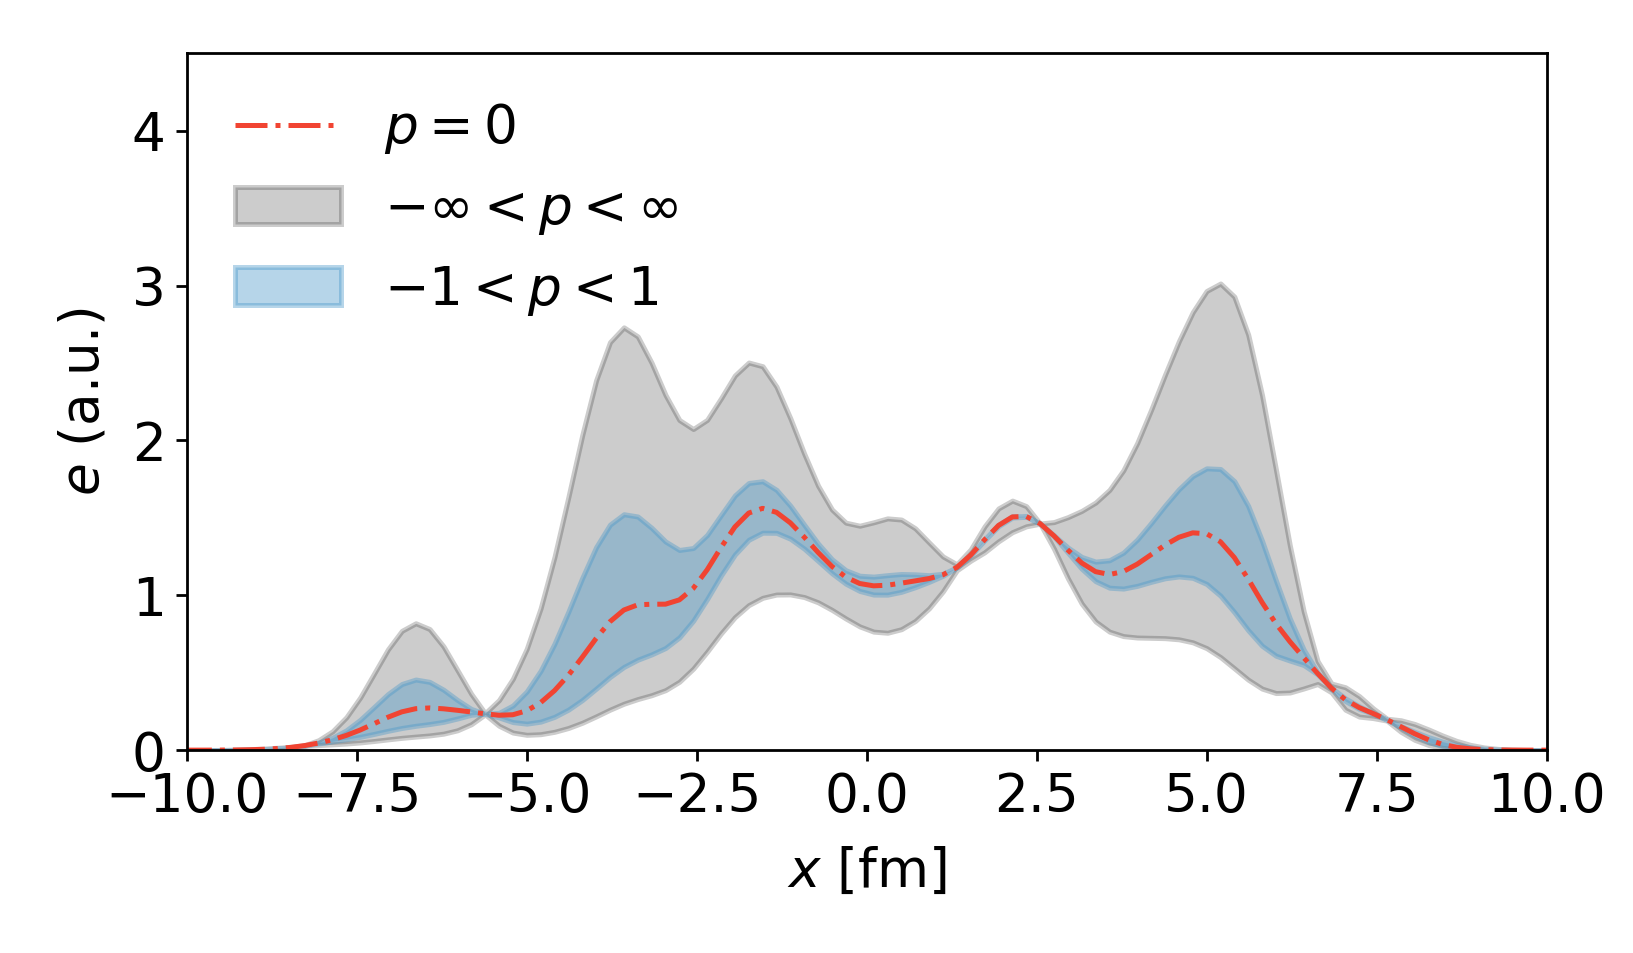
\includegraphics[width=\textwidth]{trento_p_p11.png}
\end{center}
\end{overprint}
\end{column}
\begin{column}{.7\textwidth}
\begin{itemize}
\item Energy density deposition at mid-rapidity is assumed to be a local function of participant densities:
\begin{eqnarray}
\nonumber
\frac{d E_T}{dx_\perp^2 d\eta_s}(x_\perp, \eta_s=0) = \textrm{Norm}\times f(T_A(x_\perp), T_B(x_\perp))
\end{eqnarray}
\item A particular parametric form of $f$ is used in TRENTo
\begin{overprint}
\onslide<1>
\begin{eqnarray}
\nonumber
f(T_A, T_B) = \left(\frac{T_A^p+T_B^p}{2}\right)^{1/p}
\end{eqnarray}
known as ``generalized mean'' ansatz.
\onslide<2->

\vspace{-1em}
\begin{eqnarray}
\nonumber
\left(\frac{T_A^p+T_B^p}{2}\right)^{1/p} = 
\begin{cases}
\max\{T_A, T_B\}, & p\rightarrow \infty \\
\frac{T_A+T_B}{2}, & p=1 \\
\sqrt{T_A T_B}, & p=0\\
\frac{2T_A T_B}{T_A+T_B}, & p=-1\\
\min\{T_A, T_B\}, & p\rightarrow - \infty
\end{cases}
\end{eqnarray}
$p$ parametrizes a class of {\bf initial condition uncertainty}.
\end{overprint}
\end{itemize}

\end{column}
\end{columns}
\end{frame}

\section{Event properties at the initial condition level}
\begin{frame}{Event properties}
\begin{itemize}
\item Impact-parameter: $b$.
\item Number of participants: $N_{\textrm{part}}$ nucleons that suffers at least one inelastic collisions.
\item Number of binary collisions: $N_{\textrm{coll}}$ the total number inelastic collisions.
\item Total transverse energy: $dE_T/d_\eta$ transverse summed energy per unit rapidity.
\item Eccentricity: $\epsilon_n e^{in\phi_n}$
\end{itemize}
\end{frame}

\begin{frame}{Total transverse energy: fluctuation in pp}
\begin{columns}
\begin{column}{.4\textwidth}
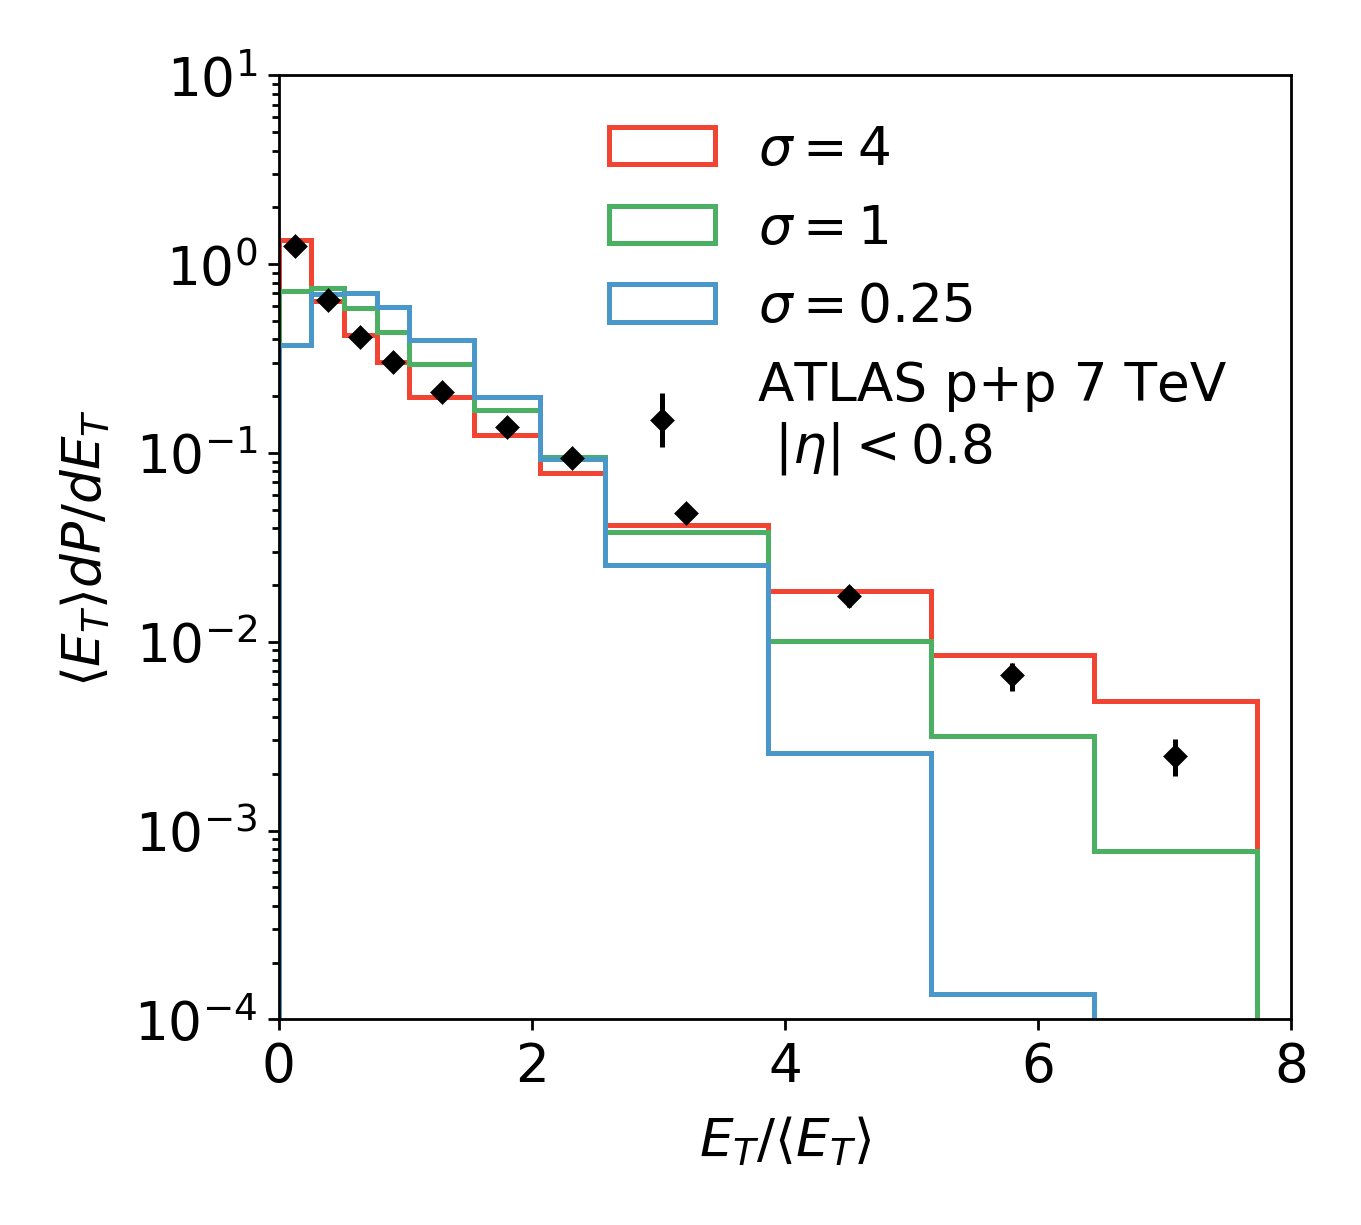
\includegraphics[width=\textwidth]{kdep.png}
\end{column}
\begin{column}{.6\textwidth}
\begin{itemize}
\item Proton-proton collision produces huge total transverse energy $E_T$,
\begin{eqnarray}
\nonumber
E_T = \sum_{|\eta_i|<0.8} e_{T,i}
\end{eqnarray}
\item Such fluctuation is both dynamic and statistical (finite acceptance).
\item In TRENTo, this is modeled by proton-proton geometry overlap + the $\Gamma$-fluctuation.
\item Important source of fluctuation in the initial condition model.
\end{itemize}
\end{column}
\end{columns}
\end{frame}

\begin{frame}{Total transverse energy: centrality dependence in AA}
\begin{itemize}
\item Different way of defining centrality at the level of initial condition:
\item[1.] Ordering events by transverse energy. With nuclear configuration and $\Gamma$-fluctuation.
\item[2.] Ordering events by number of participants. Only nuclear configuration fluctuation.
\item[3.] Ordering events by impact parameter. Least fluctuation.
\end{itemize}
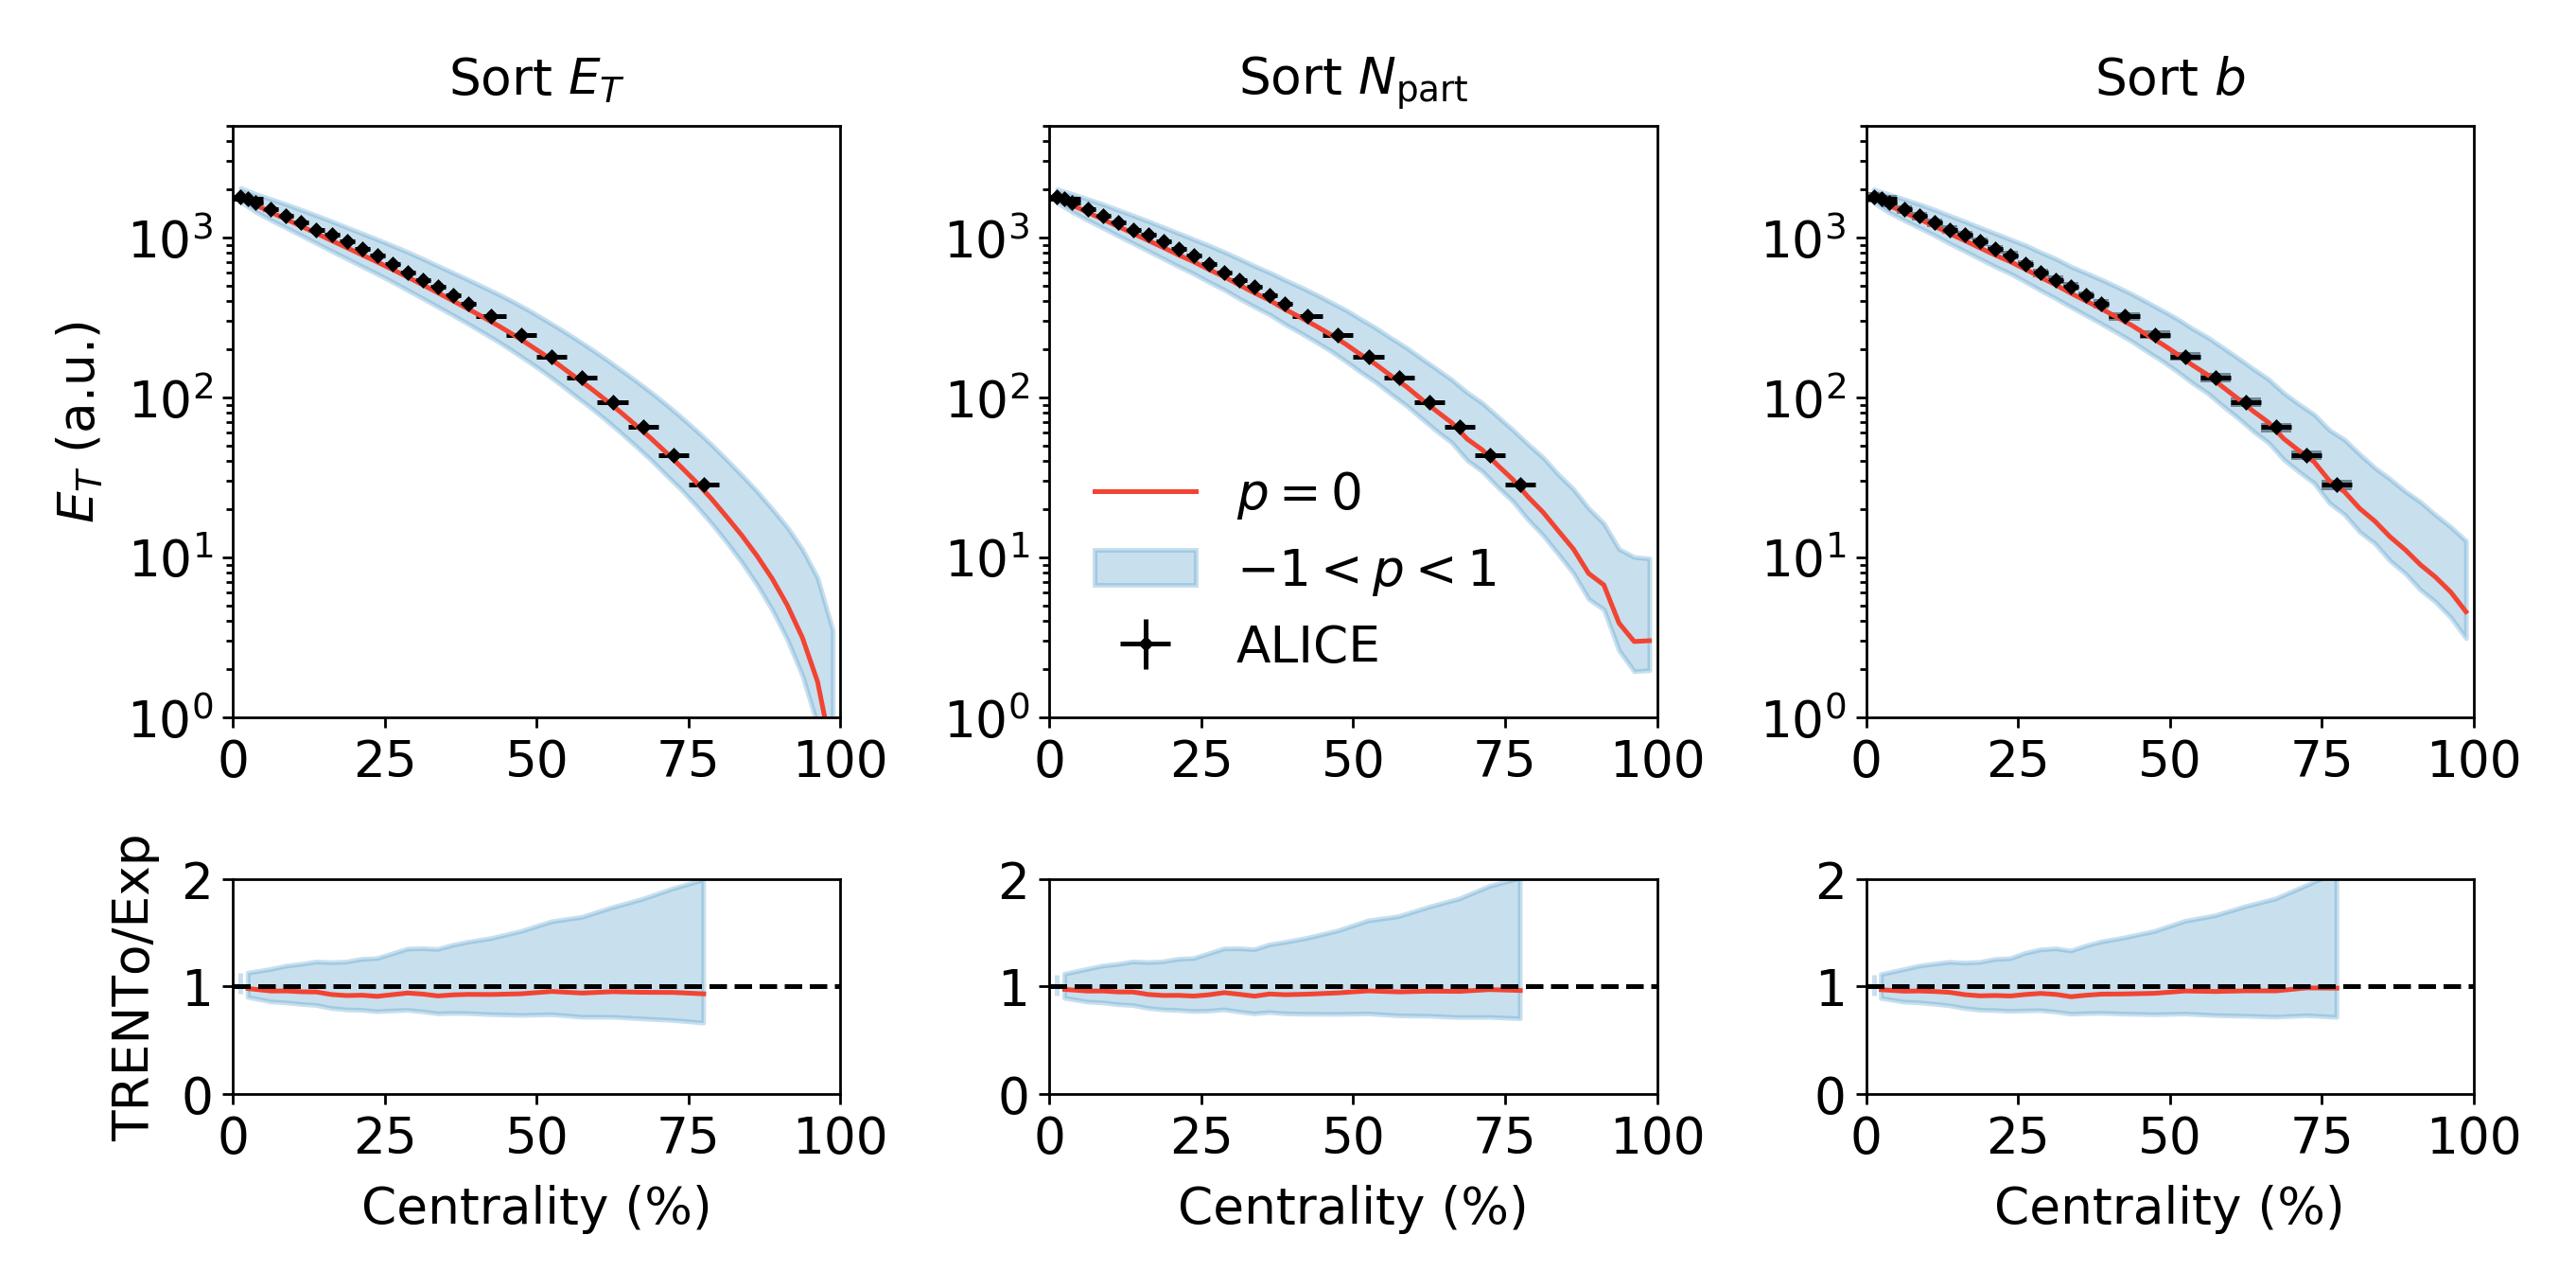
\includegraphics[width=.7\textwidth]{mult.png}
\end{frame}

\begin{frame}{Eccentricity}
\begin{columns}
\begin{column}{.4\textwidth}
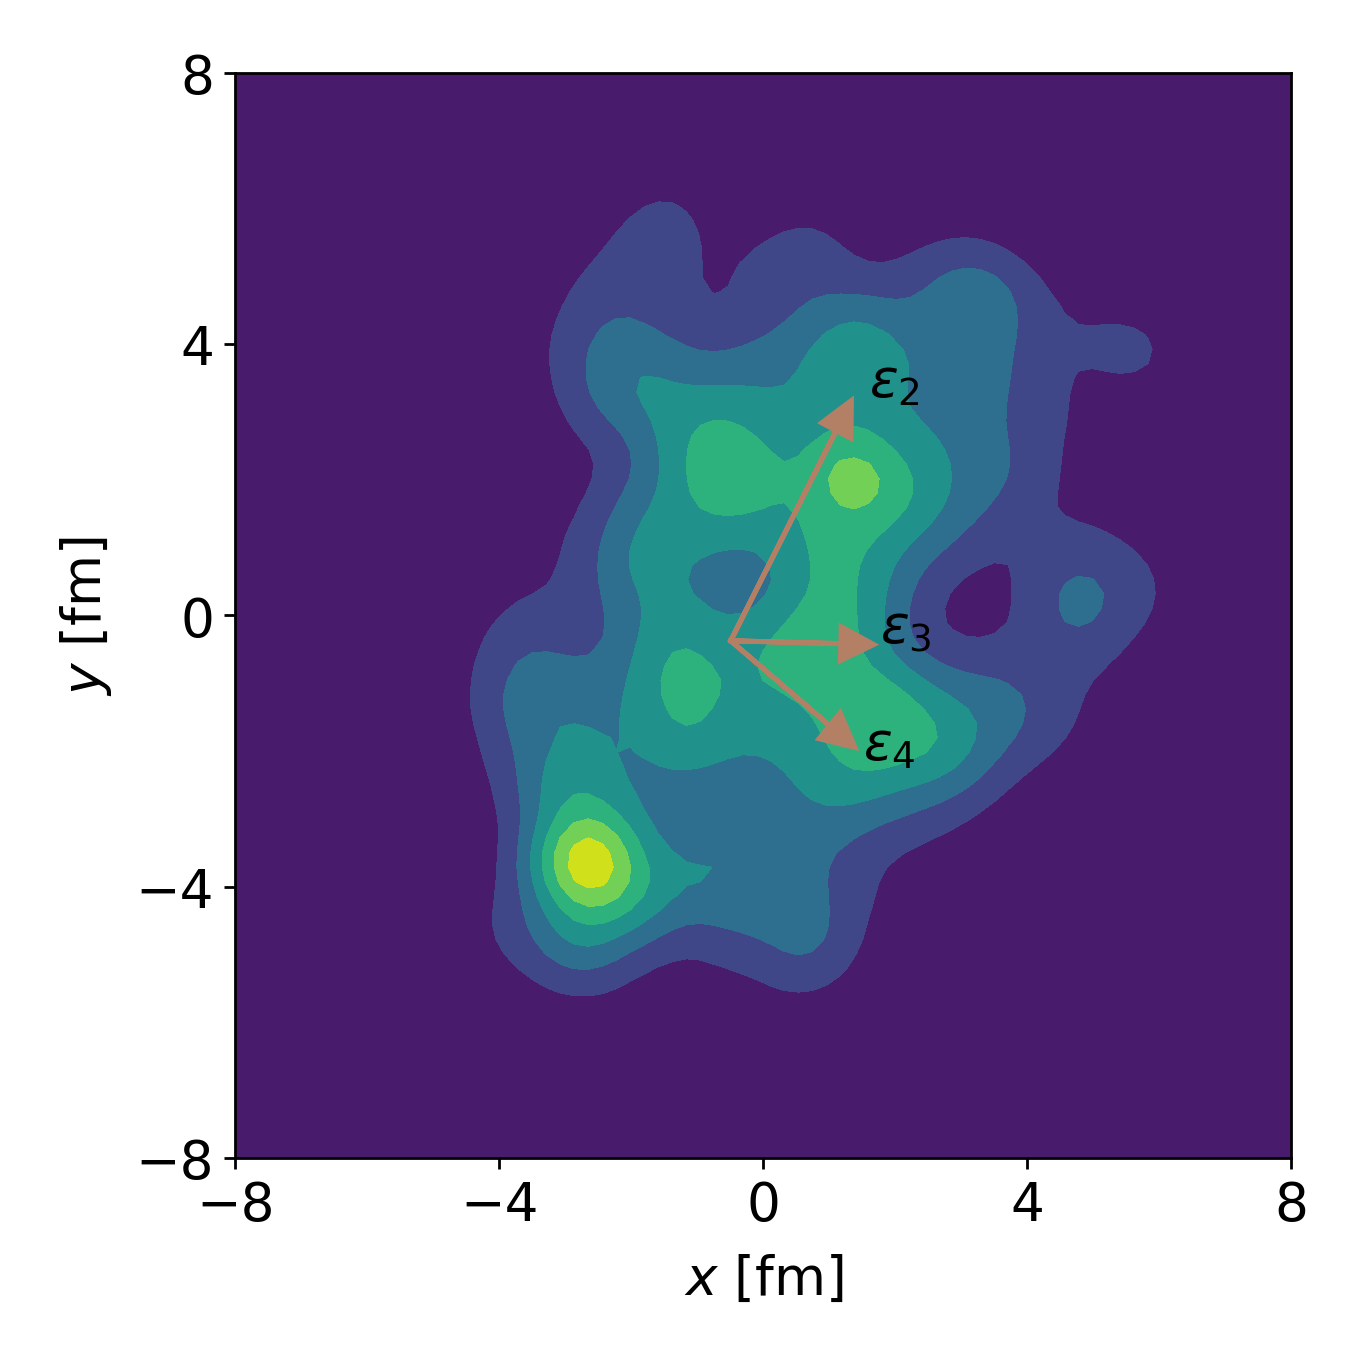
\includegraphics[width=\textwidth]{trento_demo.png}
\end{column}
\begin{column}{.6\textwidth}
\begin{itemize}
\item Finally state anisotropic flow are linear (+non-linear) responses of the hydrodynamic evolution to the initial geometric eccentricity.
\item In TRENTo, eccentricity is defined with energy density distribution $e(x, y)$.
\begin{eqnarray}
\nonumber
\epsilon_n e^{i n\phi} = \frac{\int e r^n e^{i n \phi}dx dy}{\int e r^n dx dy}
\end{eqnarray}
\end{itemize}
\end{column}
\end{columns}
\end{frame}

\begin{frame}{Eccentricity}
\begin{itemize}
\item The way energy production depends on participant density strongly affects the eccentricity of the initial nuclear geometry.
\item Notable initial condition uncertainty on the magnitude of anisotropic flow.
\end{itemize}
\begin{center}
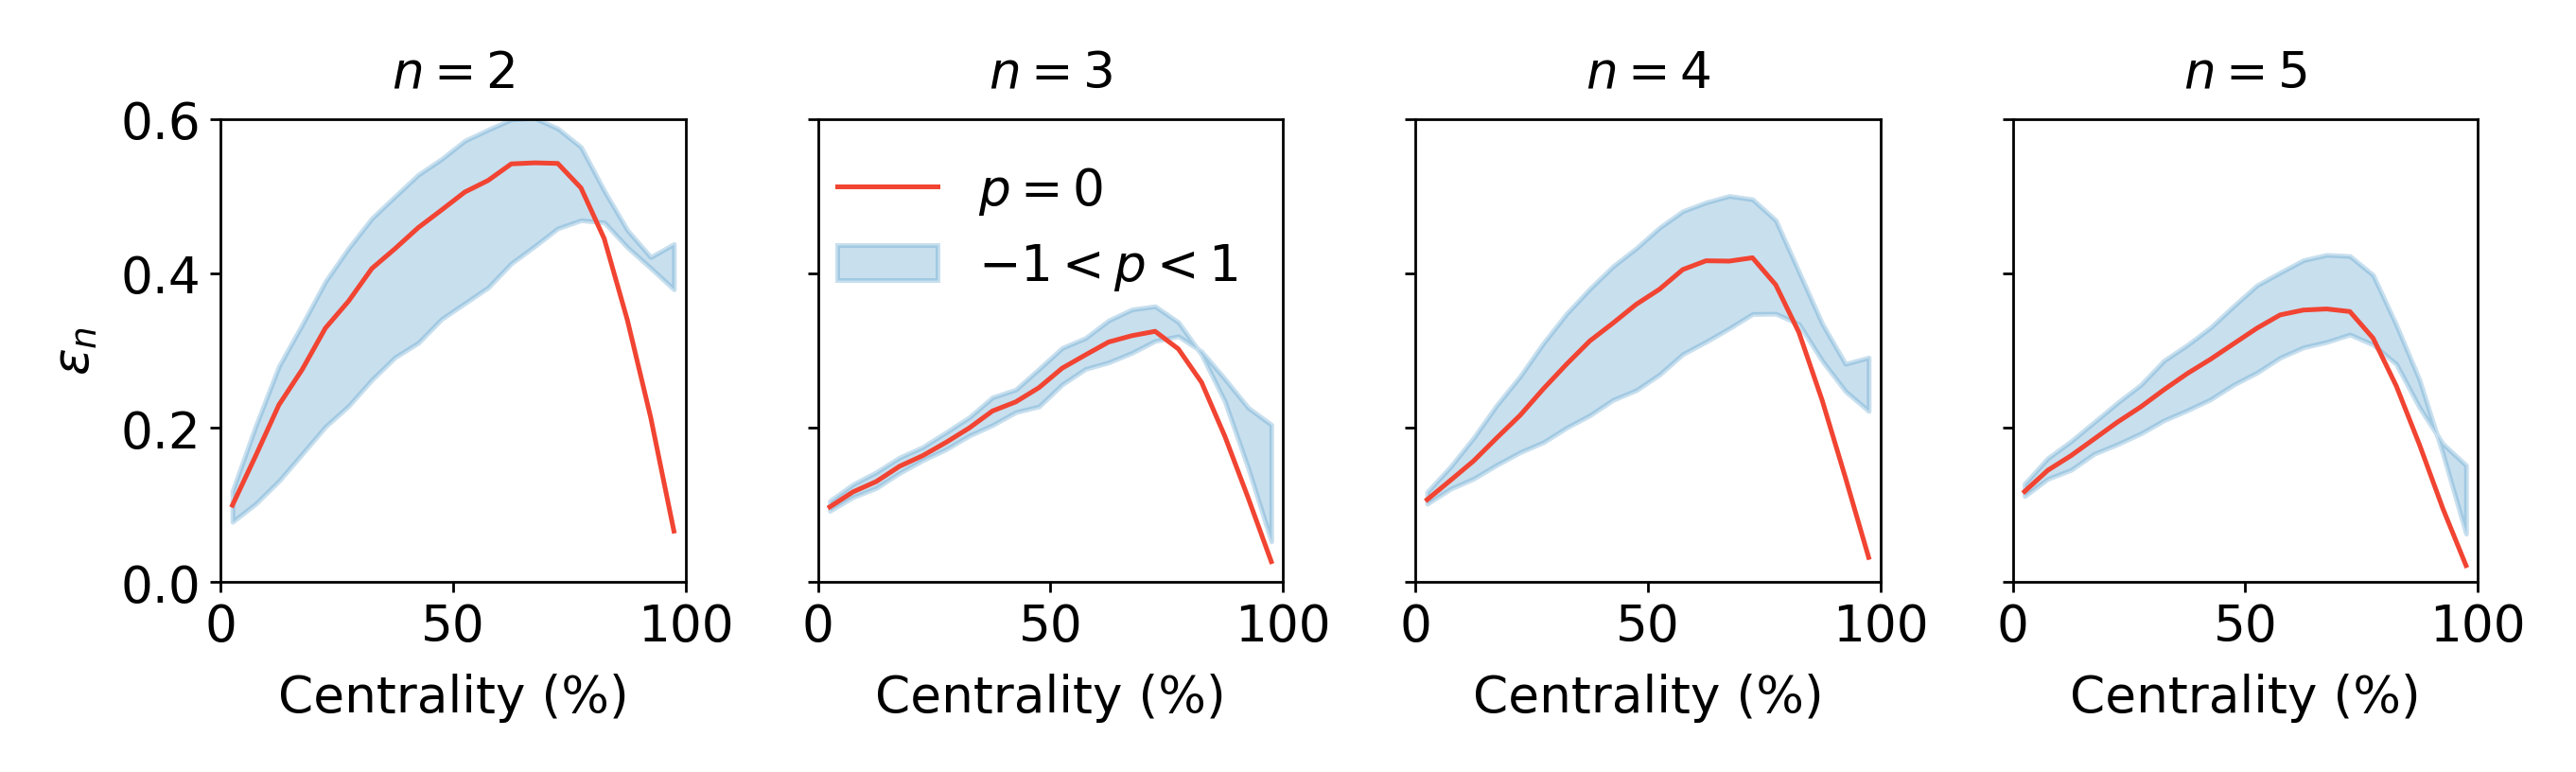
\includegraphics[width=\textwidth]{ecc.png}
\end{center}
\end{frame}

\begin{frame}{Eccentricity}
\begin{columns}
\begin{column}{.4\textwidth}
\begin{overprint}
\onslide<1>
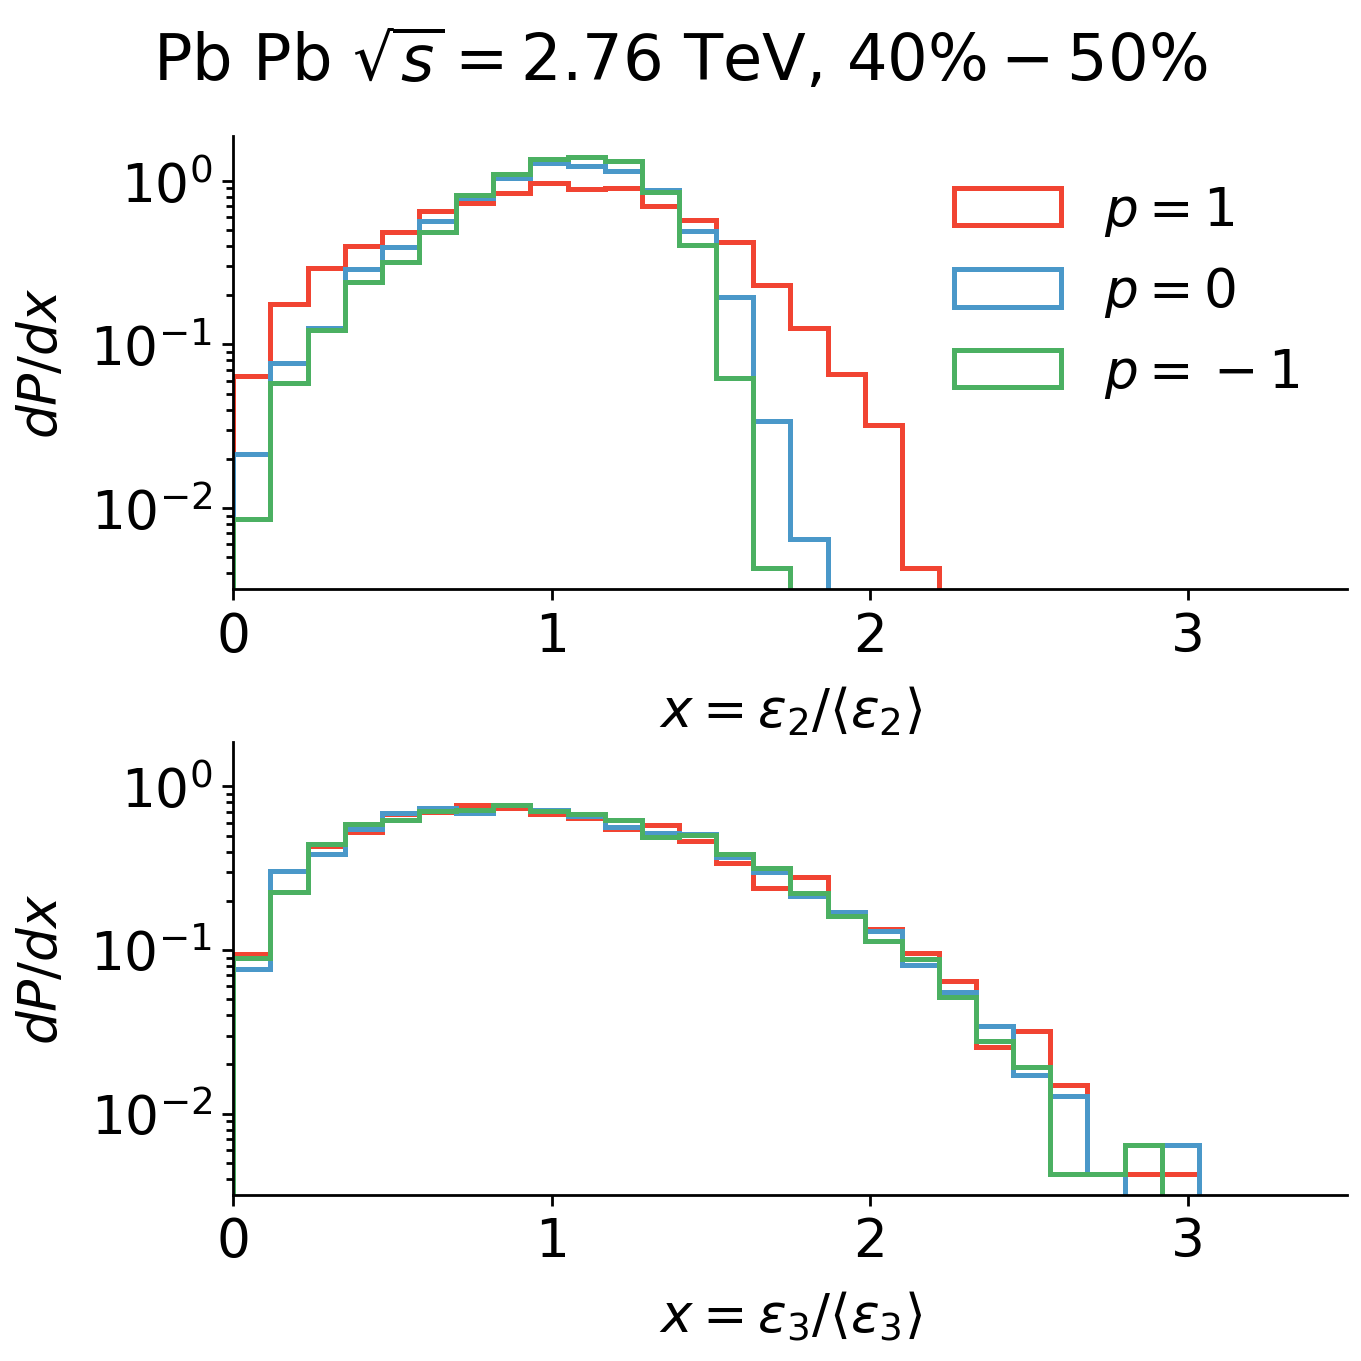
\includegraphics[width=\textwidth]{ecc_fluct_40-50.png}
\onslide<2>
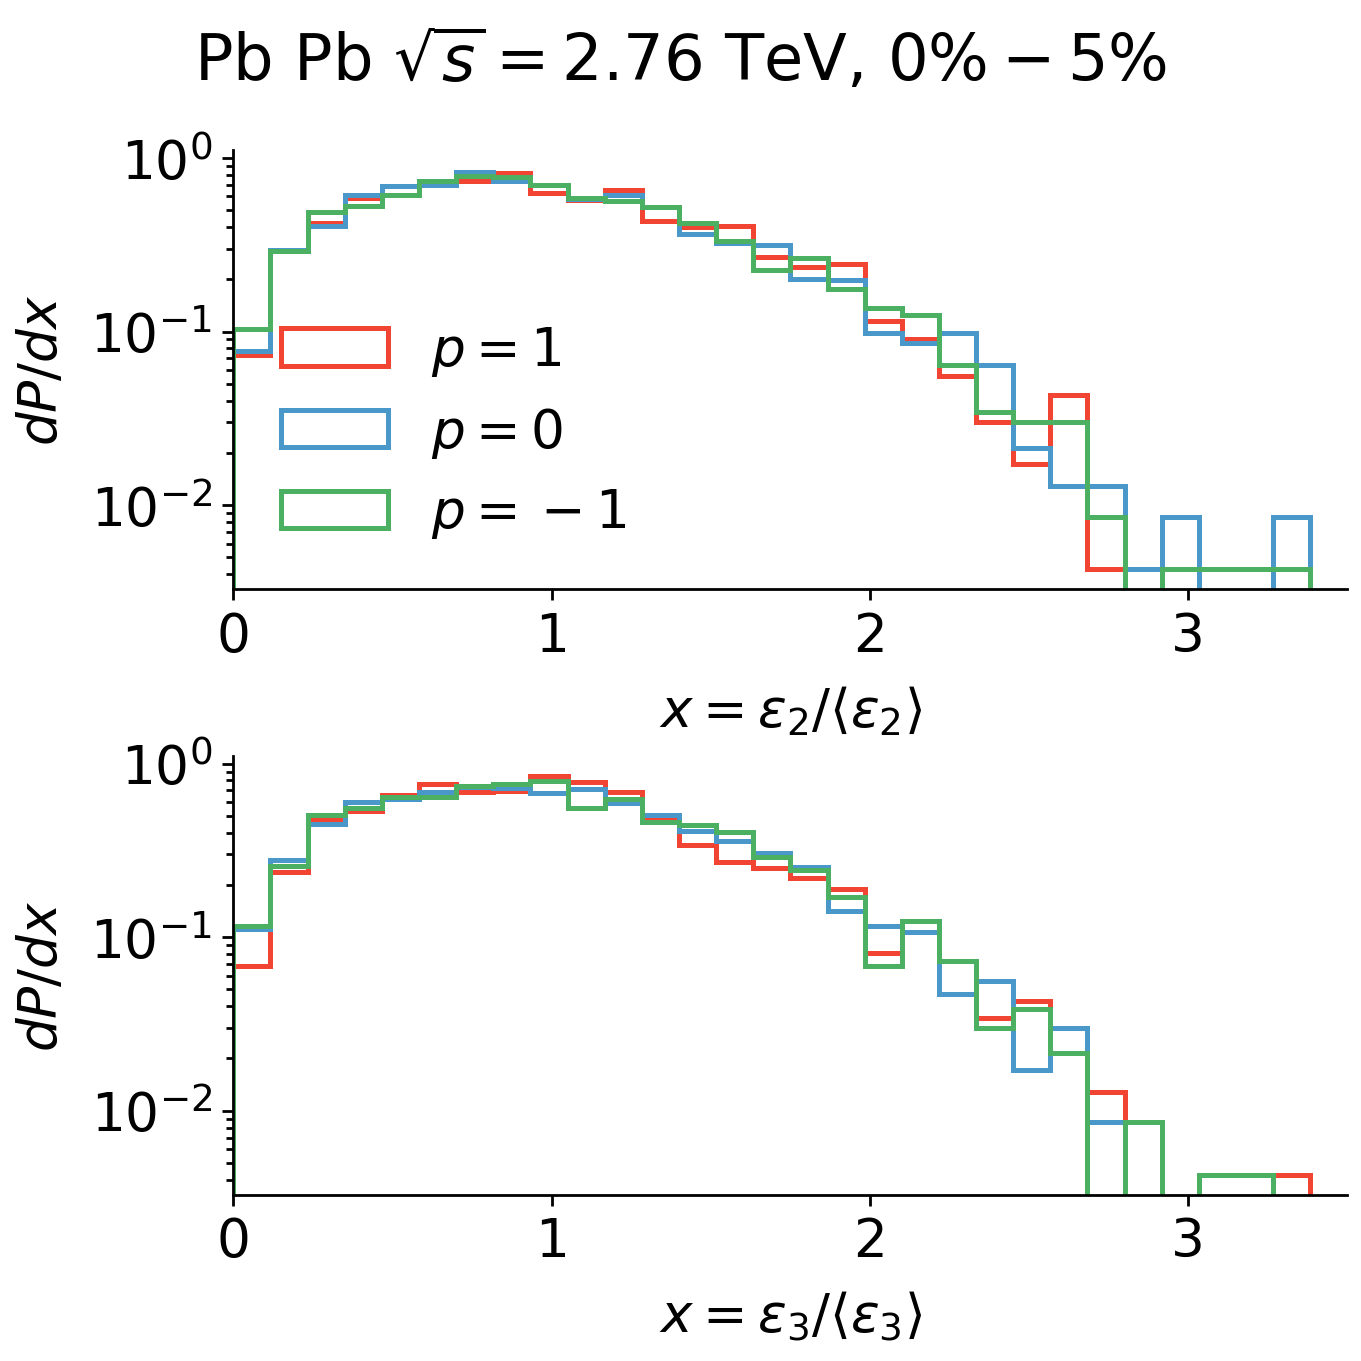
\includegraphics[width=\textwidth]{ecc_fluct_0-5.png}
\end{overprint}
\end{column}
\begin{column}{.6\textwidth}
\begin{itemize}
\item It may not be too meaningful to look at the absolute magnitude of $\epsilon_n$ in initial condition.
\item Linear reponses $v_n \sim c_n\epsilon_n +\cdots$ with unknown coefficients.\\
\item The shape of the event-by-event distribution is more directly related to initial conditions, $x=\epsilon_n/\langle \epsilon_n \rangle$
\item In $40-50\%$ centrality, $\epsilon_2$ distribution is sensitive to the energy deposition ansatz ($p$-parameter).
\item<2-> In central collisions, less-sensitive to $p$, distribution dominated by fluctuations.
\end{itemize}
\end{column}
\end{columns}
\end{frame}

\begin{frame}{Number of participants}
\begin{columns}
\begin{column}{.4\textwidth}
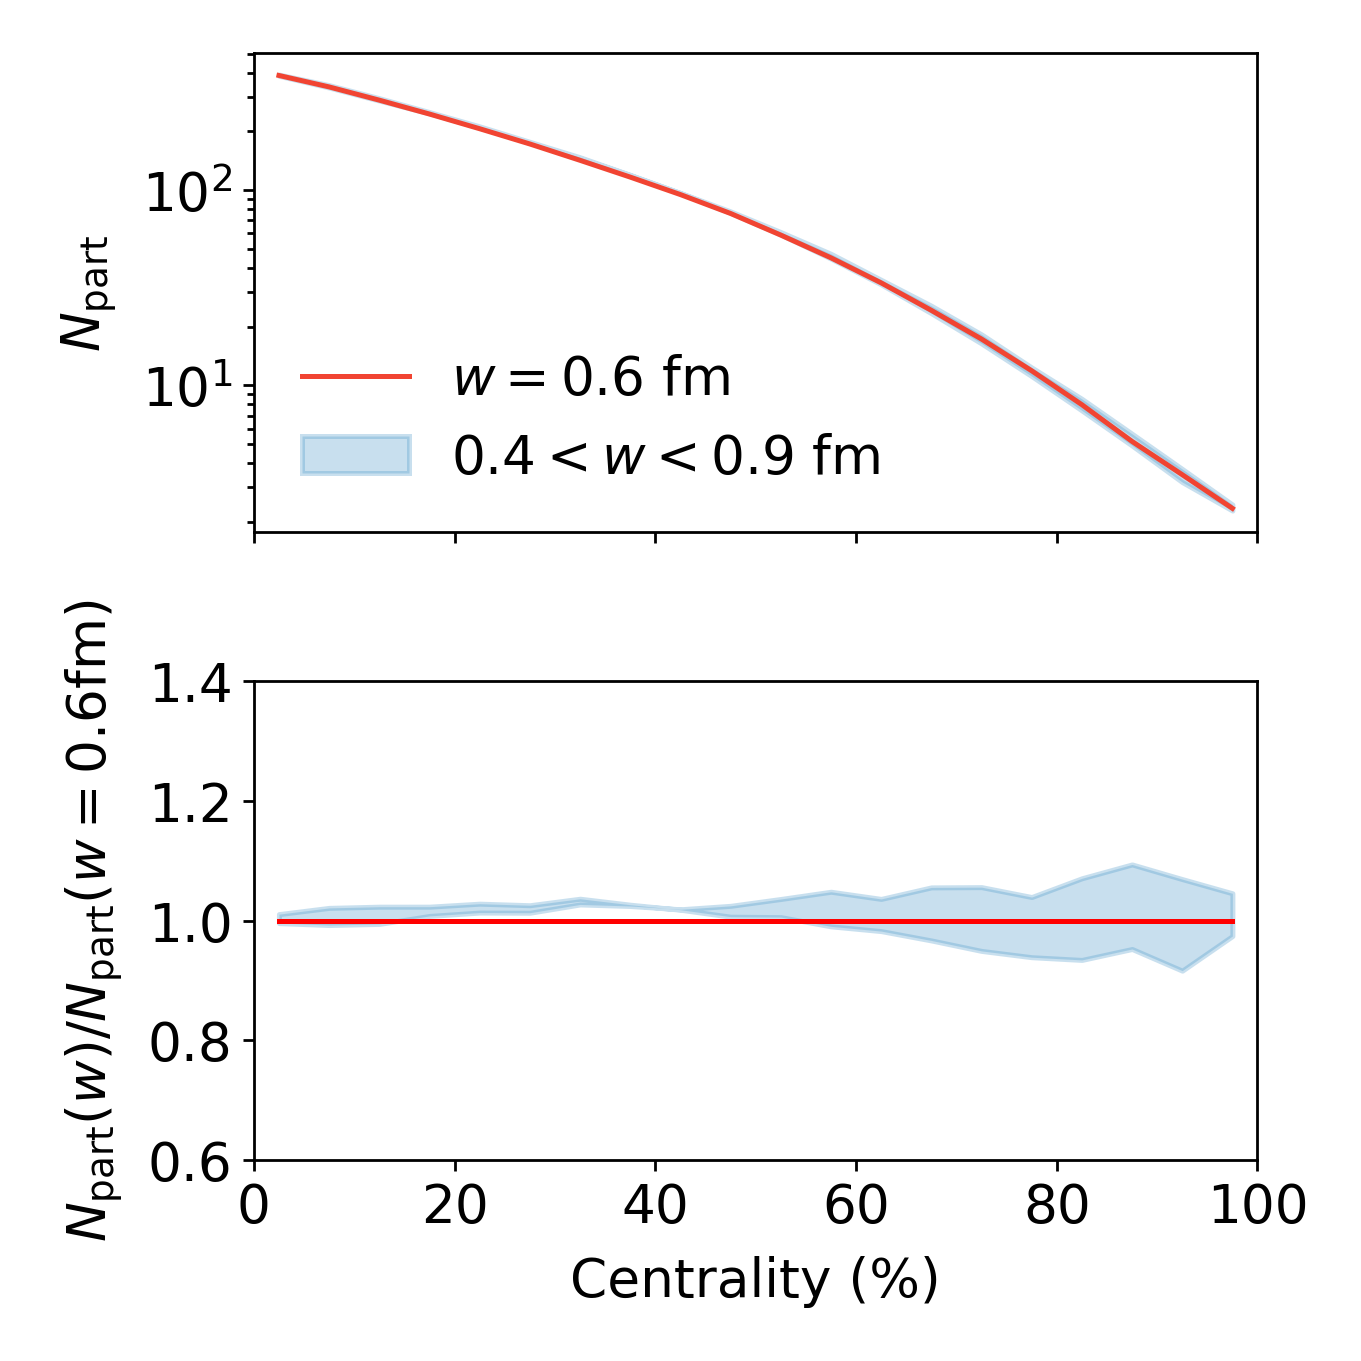
\includegraphics[width=\textwidth]{npart.png}
\end{column}
\begin{column}{.6\textwidth}
\begin{itemize}
\item Number of participants is rather insensitive to the size of proton.
\item Probability for a nucleon "i" to be a participant depends on the overlap of the proton density and the thickness of the whole other nuclei $T_{pA}$.
\begin{eqnarray}
\nonumber
&&1 -\prod_j (1-P_{\textrm{coll}}(b_{ij}))=1-e^{-\sigma_{gg}\sum_j T_{pp}(b_{ij})}\\\nonumber
&\approx & 1-\exp\left\{- \# f(\frac{\sigma_{NN}}{w^2}) w^2 T_{pA}\right\}
\end{eqnarray}
\item For large nuclei, a different nucleon width only affects this probability at the boundary, so $N_{\textrm{part}}$ is not sensitive to $w$.
\end{itemize}
\end{column}
\end{columns}
\end{frame}

\begin{frame}{Number of binary collisions}
\begin{columns}
\begin{column}{.4\textwidth}
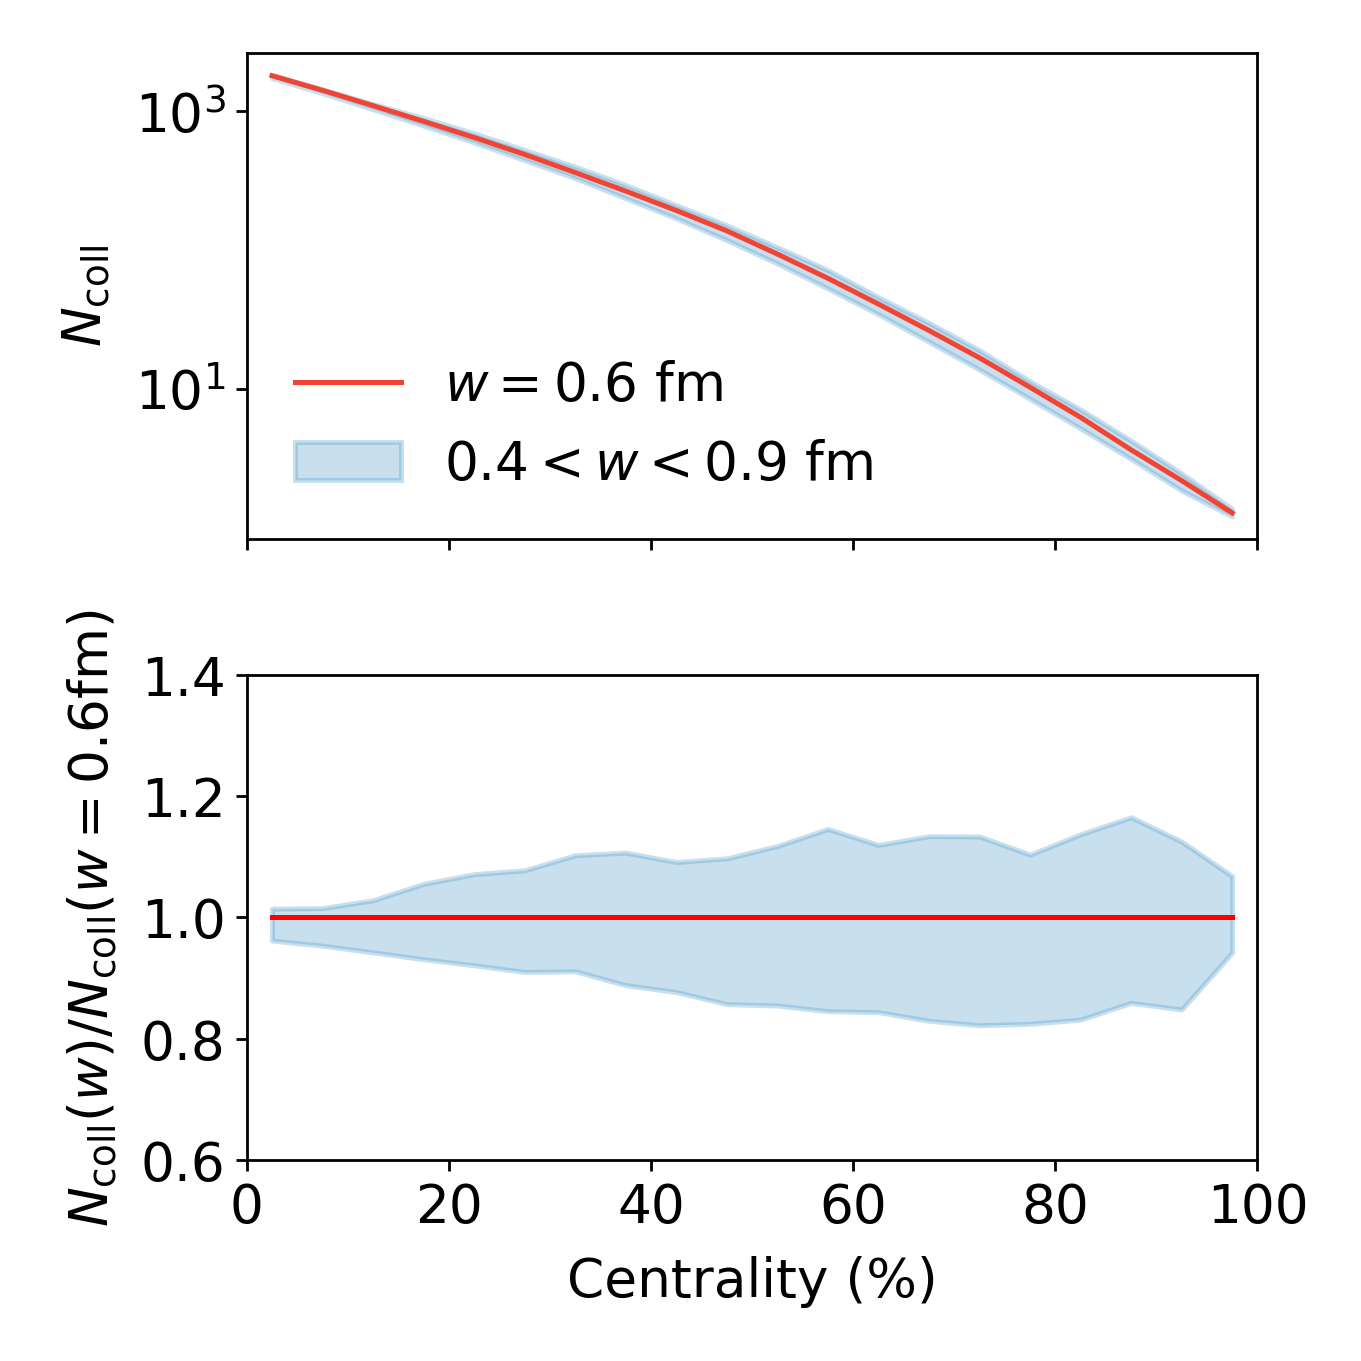
\includegraphics[width=\textwidth]{ncoll.png}
\end{column}
\begin{column}{.6\textwidth}
\begin{itemize}
\item Number of binary collisions: a measure of \# of hard process (tiny fraction of the inelastic collision) in AA collisions.
\item It is determined by $T_{pp}$,
\begin{eqnarray}
\nonumber
N_{\textrm{coll}} = \left\langle \sum_{i\in A, j\in B} 
\left(1-e^{
-\frac{1}{4\pi}f\left(\frac{\sigma_{NN}}{w^2}\right)e^{-\frac{b_{ij}^2}{4w^2}}
}\right)
\right\rangle
\end{eqnarray}
\item Sensitive to proton-proton overlap, and therefore sensitive to nucleon width parameter $w$.
\end{itemize}
\end{column}
\end{columns}
\end{frame}

\section{Program installation and usage}
\begin{frame}[fragile]{Installation and usage (standalone)}
\begin{itemize}
\item Language: {\tt c++}
\item Dependence: {\tt boost, hdf5, gsl, c++11}
\item Download: 
\begin{lstlisting}
$ git clone https://github.com/Duke-QCD/trento.git
\end{lstlisting}
\item Build and install (default path \$HOME/.local)
\begin{lstlisting}
$ mkdir build &&  cd build
$ cmake ..
$ make install
\end{lstlisting}
\item Usage 
\begin{lstlisting}[language=bash]
$ trento [options] projectile target [number-events = 1]
\end{lstlisting}
\end{itemize}
\end{frame}



\begin{frame}[fragile]{Usage (standalone)}

Example: generate 3 ``minimum bias'' Pb+Pb collisions.
\begin{lstlisting}[language=bash]
trento Pb Pb 3
\end{lstlisting}
A subset of options:
\begin{itemize}
\item Nuclei: p, d, Cu, Xe, Au, Pb, U
\item Nuclear configuration:
\begin{itemize}
\item "-w": width [fm] of the Gaussian shape of the proton $\frac{1}{2\pi w^2}e^{-r^2/(2w^2)}$.
\item "-d": minimum nucleon distance [fm], short-range repulsion.
\item "-k": nucleonic fluctuation. Unit-mean $\Gamma$ distribution, with variance $\sigma=1/k^2$.
\end{itemize}
\item Collision
\begin{itemize}
\item "-x": set $\sigma_{pp}^{\textrm{inel}}~[\mathrm{fm}^2]$, $\sim 4.2~\mathrm{fm}^2$ @200 GeV, $6.4~\mathrm{fm}^2$@2.76 TeV, $7.0~\mathrm{fm}^2$ @ 5 TeV.
\item "{\tt--}ncoll": compute binary collision number (slow down the program a little).
\end{itemize}
\item Energy deposition
\begin{itemize}
\item "-p": set the $p$ value in energy deposition ansatz $\sim (T_A^p+T_B^p)^{1/p}$.
\end{itemize}
\end{itemize}

\end{frame}

\section{Summary and exercises }
\begin{frame}{Summary}
\begin{itemize}
\item The soft sector initial condition in JETSCAPE uses a parametric model TRENTo.
\item Initial condition is big source of uncertainty for understanding soft-sector evolution quantitatively from data.
\item TRENTo parametrizes major uncertainties such as,
\begin{itemize}
\item Energy deposition relation at mid-rapidity.
\item Uncertainty in proton width and fluctuation.
\item Nucleon substructure and rapidity-dependence (not mentioned in this lecture).
\end{itemize}
\end{itemize}

\end{frame}

\begin{frame}{Hands-on exercises for Bayesian model calibration:}
\begin{itemize}
\item[1.] Use one single dataset of $E_T$ measurement to infer the initial condition parameters I used to generated the data.
\item[2.] Add one more dataset $P(\epsilon_n/\langle \epsilon_n\rangle)$, how does it improves the parameter inference?
\item[3.] Apply the procedure to real measurements of $E_T$, and $P(v_n/\langle v_n\rangle)$ (use $P(\epsilon_n/\langle \epsilon_n\rangle)$ as a first approximation). What does experimental data reveal?
\item[4.] How to estimate the uncertainty stems from our over-simplified model of $P(v_n/\langle v_n\rangle)\approx P(\epsilon_n/\langle \epsilon_n\rangle)$?
\end{itemize}
\end{frame}
\end{document}
